% Options for packages loaded elsewhere
\PassOptionsToPackage{unicode}{hyperref}
\PassOptionsToPackage{hyphens}{url}
\PassOptionsToPackage{dvipsnames,svgnames,x11names}{xcolor}
%
\documentclass[
]{article}
\usepackage{amsmath,amssymb}
\usepackage{iftex}
\ifPDFTeX
  \usepackage[T1]{fontenc}
  \usepackage[utf8]{inputenc}
  \usepackage{textcomp} % provide euro and other symbols
\else % if luatex or xetex
  \usepackage{unicode-math} % this also loads fontspec
  \defaultfontfeatures{Scale=MatchLowercase}
  \defaultfontfeatures[\rmfamily]{Ligatures=TeX,Scale=1}
\fi
\usepackage{lmodern}
\ifPDFTeX\else
  % xetex/luatex font selection
\fi
% Use upquote if available, for straight quotes in verbatim environments
\IfFileExists{upquote.sty}{\usepackage{upquote}}{}
\IfFileExists{microtype.sty}{% use microtype if available
  \usepackage[]{microtype}
  \UseMicrotypeSet[protrusion]{basicmath} % disable protrusion for tt fonts
}{}
\makeatletter
\@ifundefined{KOMAClassName}{% if non-KOMA class
  \IfFileExists{parskip.sty}{%
    \usepackage{parskip}
  }{% else
    \setlength{\parindent}{0pt}
    \setlength{\parskip}{6pt plus 2pt minus 1pt}}
}{% if KOMA class
  \KOMAoptions{parskip=half}}
\makeatother
\usepackage{xcolor}
\usepackage[margin=1in]{geometry}
\usepackage{color}
\usepackage{fancyvrb}
\newcommand{\VerbBar}{|}
\newcommand{\VERB}{\Verb[commandchars=\\\{\}]}
\DefineVerbatimEnvironment{Highlighting}{Verbatim}{commandchars=\\\{\}}
% Add ',fontsize=\small' for more characters per line
\usepackage{framed}
\definecolor{shadecolor}{RGB}{248,248,248}
\newenvironment{Shaded}{\begin{snugshade}}{\end{snugshade}}
\newcommand{\AlertTok}[1]{\textcolor[rgb]{0.94,0.16,0.16}{#1}}
\newcommand{\AnnotationTok}[1]{\textcolor[rgb]{0.56,0.35,0.01}{\textbf{\textit{#1}}}}
\newcommand{\AttributeTok}[1]{\textcolor[rgb]{0.13,0.29,0.53}{#1}}
\newcommand{\BaseNTok}[1]{\textcolor[rgb]{0.00,0.00,0.81}{#1}}
\newcommand{\BuiltInTok}[1]{#1}
\newcommand{\CharTok}[1]{\textcolor[rgb]{0.31,0.60,0.02}{#1}}
\newcommand{\CommentTok}[1]{\textcolor[rgb]{0.56,0.35,0.01}{\textit{#1}}}
\newcommand{\CommentVarTok}[1]{\textcolor[rgb]{0.56,0.35,0.01}{\textbf{\textit{#1}}}}
\newcommand{\ConstantTok}[1]{\textcolor[rgb]{0.56,0.35,0.01}{#1}}
\newcommand{\ControlFlowTok}[1]{\textcolor[rgb]{0.13,0.29,0.53}{\textbf{#1}}}
\newcommand{\DataTypeTok}[1]{\textcolor[rgb]{0.13,0.29,0.53}{#1}}
\newcommand{\DecValTok}[1]{\textcolor[rgb]{0.00,0.00,0.81}{#1}}
\newcommand{\DocumentationTok}[1]{\textcolor[rgb]{0.56,0.35,0.01}{\textbf{\textit{#1}}}}
\newcommand{\ErrorTok}[1]{\textcolor[rgb]{0.64,0.00,0.00}{\textbf{#1}}}
\newcommand{\ExtensionTok}[1]{#1}
\newcommand{\FloatTok}[1]{\textcolor[rgb]{0.00,0.00,0.81}{#1}}
\newcommand{\FunctionTok}[1]{\textcolor[rgb]{0.13,0.29,0.53}{\textbf{#1}}}
\newcommand{\ImportTok}[1]{#1}
\newcommand{\InformationTok}[1]{\textcolor[rgb]{0.56,0.35,0.01}{\textbf{\textit{#1}}}}
\newcommand{\KeywordTok}[1]{\textcolor[rgb]{0.13,0.29,0.53}{\textbf{#1}}}
\newcommand{\NormalTok}[1]{#1}
\newcommand{\OperatorTok}[1]{\textcolor[rgb]{0.81,0.36,0.00}{\textbf{#1}}}
\newcommand{\OtherTok}[1]{\textcolor[rgb]{0.56,0.35,0.01}{#1}}
\newcommand{\PreprocessorTok}[1]{\textcolor[rgb]{0.56,0.35,0.01}{\textit{#1}}}
\newcommand{\RegionMarkerTok}[1]{#1}
\newcommand{\SpecialCharTok}[1]{\textcolor[rgb]{0.81,0.36,0.00}{\textbf{#1}}}
\newcommand{\SpecialStringTok}[1]{\textcolor[rgb]{0.31,0.60,0.02}{#1}}
\newcommand{\StringTok}[1]{\textcolor[rgb]{0.31,0.60,0.02}{#1}}
\newcommand{\VariableTok}[1]{\textcolor[rgb]{0.00,0.00,0.00}{#1}}
\newcommand{\VerbatimStringTok}[1]{\textcolor[rgb]{0.31,0.60,0.02}{#1}}
\newcommand{\WarningTok}[1]{\textcolor[rgb]{0.56,0.35,0.01}{\textbf{\textit{#1}}}}
\usepackage{longtable,booktabs,array}
\usepackage{calc} % for calculating minipage widths
% Correct order of tables after \paragraph or \subparagraph
\usepackage{etoolbox}
\makeatletter
\patchcmd\longtable{\par}{\if@noskipsec\mbox{}\fi\par}{}{}
\makeatother
% Allow footnotes in longtable head/foot
\IfFileExists{footnotehyper.sty}{\usepackage{footnotehyper}}{\usepackage{footnote}}
\makesavenoteenv{longtable}
\usepackage{graphicx}
\makeatletter
\def\maxwidth{\ifdim\Gin@nat@width>\linewidth\linewidth\else\Gin@nat@width\fi}
\def\maxheight{\ifdim\Gin@nat@height>\textheight\textheight\else\Gin@nat@height\fi}
\makeatother
% Scale images if necessary, so that they will not overflow the page
% margins by default, and it is still possible to overwrite the defaults
% using explicit options in \includegraphics[width, height, ...]{}
\setkeys{Gin}{width=\maxwidth,height=\maxheight,keepaspectratio}
% Set default figure placement to htbp
\makeatletter
\def\fps@figure{htbp}
\makeatother
\setlength{\emergencystretch}{3em} % prevent overfull lines
\providecommand{\tightlist}{%
  \setlength{\itemsep}{0pt}\setlength{\parskip}{0pt}}
\setcounter{secnumdepth}{-\maxdimen} % remove section numbering
\usepackage{amsmath}
\usepackage{optidef}
\usepackage{accents}
\usepackage{caption}
\ifLuaTeX
  \usepackage{selnolig}  % disable illegal ligatures
\fi
\usepackage{bookmark}
\IfFileExists{xurl.sty}{\usepackage{xurl}}{} % add URL line breaks if available
\urlstyle{same}
\hypersetup{
  pdftitle={Problem Set 6: Estimation of TEs Using Matching Methods},
  pdfauthor={Tessie Dong, Derek Li, Andi Liu},
  colorlinks=true,
  linkcolor={Maroon},
  filecolor={Maroon},
  citecolor={Blue},
  urlcolor={Blue},
  pdfcreator={LaTeX via pandoc}}

\title{Problem Set 6: Estimation of TEs Using Matching Methods}
\author{Tessie Dong, Derek Li, Andi Liu}
\date{Due Feb 1st, 2024}

\begin{document}
\maketitle

\noindent \textcolor{Maroon}{\textbf{Objective}: In PSet 5 you used the \texttt{nswpsid.csv} data to estimate the \textcolor{ForestGreen}{propensity score (pscore)}, i.e., the probability that a unit is assigned to treatment as a function of their observed pre-determined characteristics (OPVs). You employed three estimation approaches: 1) OLS applied to a \textcolor{ForestGreen}{Linear Probability Model (LPM)}; 2) \textcolor{ForestGreen}{Lasso} also applied to a LPM; and, 3) \textcolor{ForestGreen}{Maximum Likelihood Estimation (MLE)} applied to a \textcolor{ForestGreen}{Logit Model}. In this PSet you use the Logit-based estimates of the pscore to estimate the ATT (of the offer of training) on post-training earning using four pscore-based matching approaches: 1) \textcolor{ForestGreen}{(Naive) Stratification Matching (SM)}; 2) \textcolor{ForestGreen}{Nearest-neighbor Matching (NNM)}; 3) \textcolor{ForestGreen}{Radius Matching (RM)}; and, 4) \textcolor{ForestGreen}{Kernel Matching (KM)}.} \\


\noindent \textcolor{Maroon}{\textbf{Background}: All matching approaches are predicated on the \textcolor{ForestGreen}{conditional independence assumption (CIA)} holding, i.e., on the assumption that \textit{conditional} on observed pre-determined characteristics (OPVs) treatment is as good as randomly assigned. When CIA holds, we can in theory exactly match (i.e., pair) treated and control units based on their OPVs, then estimate the treatment effect on the treated as the difference in the average outcome of the treated and the average outcome of the matched controls. This estimator will not be confounded by differences in OPVs because the \textcolor{ForestGreen}{matched sample} is by construction exactly balanced in the pre-treatment characteristics.} \\

\noindent \textcolor{Maroon}{In practice, matching exactly on OPVs runs into the \textcolor{ForestGreen}{curse of dimensionality problem} whenever there are many OPVs and/or some OPVs take many values. The statisticians Rosenbaum and Rubin (1983) showed that identification of TEs under CIA does not hinge on matching exactly on OPVs because imbalance in the OPVs matter only as far as it produces imbalance in the pscores. That is, matching units with different OPVs but the same pscore suffices to identify TEs. Formally, their result says that if CIA holds, then the potential outcomes are independent of treatment status conditional on the pscore.} \\

\noindent \textcolor{Maroon}{Rosembaum and Rubin's result suggests a matching estimator that matches controls to treated units based on the pscore rather than directly on the OPVs. In practice, matching exactly on the pscore may face the problem that there is no control unit with the same pscore value as a treated unit's (or viceversa). Econometricians have developed matching techniques to overcome this problem. These techniques differ in their implementation details but they share the same basic idea: instead of matching a control unit and a treated unit only when they have the exact same value of the pscore, they are matched if their pscores are ``sufficiently similar.'' The various techniques differ in terms of which matches they regard as ``sufficiently similar.'' As mentioned above, in this Pset you consider and implement four such techniques, i.e., SM, NNM, RM, and KM.} \\

\noindent \textcolor{Maroon}{Here is the gist of each technique: 
\begin{itemize}
\item \textbf{SM}: The idea of stratification is to divide the range of variation of the pscore into intervals such that within each interval there are both treated and control units and they have, \textit{on average}, the same pscore. In the limit, i.e., as we increase the number of intervals along with the sample size, SM matches exactly on the pscore. \item \textbf{NNM}: The idea of nearest-neighbor matching is to match a treated unit with the ``nearest'' M control units (M could be just 1 or a number larger than one). The control units matched to a treated unit are called the treated unit's ``nearest neighbors.'' In the limit, i.e., as we increase the sample size to infinity, NNM matches exactly on the pscore. 
\item \textbf{RM}: Each treated unit is matched with the control units whose pscore falls within a predefined neighborhood of the pscore of the treated unit. If the dimension of the neighborhood (i.e., the radius) is set very small, it is possible that some treated units are not matched because the neighborhood does not contain control units. On the other hand, the smaller the size of the neighborhood, the better the quality of the resulting matches. In the limit, i.e., as we decrease the radius along with increases in the sample size, RM matches exactly on the pscore. 
\item \textbf{KM}: Each treated unit is matched with a weighted average of all control units with weights that are inversely proportional to the difference between the pscore of the treated unit and that of the control units. In the limit, i.e., as we decrease the bandwith along with increases in the sample size, KM matches exactly on the pscore.
\end{itemize}
 In finite samples, the above four techniques reach different points on the frontier of the trade-off between quality and quantity of the matches, and none of them is a priori superior.}


\newpage

\subsection{Part 1: Naive Stratification Matching on the Propensity
Score (50
Points)}\label{part-1-naive-stratification-matching-on-the-propensity-score-50-points}

\noindent \textcolor{Maroon}{\textbf{Background: Common Support and Trimming}. Let $\widehat{p}_i$ denote the estimate of the pscore for unit $i$. Let $\left(\widehat{p}^{C,l},\widehat{p}^{C,u}\right)$ denote the smallest (``lower'') and largest (``upper'') $\widehat{p}_{i}$ among control units and $\left(\widehat{p}^{T,l},\widehat{p}^{T,u}\right) $ the smallest and largest $\widehat{p}_{i}$ among treated units. The range $\left[\max \left\{ \widehat{p}^{C,l},\widehat{p}^{T,l}\right\},\min \left\{ \widehat{p}^{C,u},\widehat{p}^{T,u}\right\} \right] $ is called the \textcolor{ForestGreen}{common support}. To understand this terminology observe that $\left(\widehat{p}^{C,l},\widehat{p}^{C,u}\right)$ are the extremes of the support of the empirical distribution of the pscore among the controls and $\left(\widehat{p}^{T,l},\widehat{p}^{T,u}\right) $ are the extremes of the support of the empirical distribution of the pscore among the treated; the common support is the intersection of the two empirical supports. By definition, a treated unit whose pscore is outside of the common support has no exact match among the control units and viceversa. \textcolor{ForestGreen}{Trimming} is a procedure whereby we drop sample units. There are various ways of implementing trimming for the purpose of pscore matching. A common approach is to drop all units (control and treated alike) whose $\widehat{p}_{i}$ falls outside of the common support.}


\begin{enumerate}
\def\labelenumi{\arabic{enumi}.}
\tightlist
\item
  (5 p) Let \(\widehat{p}_i\) denote the Logit-based estimate of the
  pscore for unit \(i\) which you obtained in PSet 5. Drop all sample
  units whose \(\widehat{p}_{i}\) falls outside of the common support.
  Why may a researcher want to trim the sample in this way? How many
  control (treated) units do you drop? Are you surprised? In all
  subsequent questions you use the resulting
  \textcolor{ForestGreen}{trimmed sample}.
  \textcolor{gray}{\textbf{Programming Guidance:} Use \texttt{dplyr::filter()} to drop rows from a dataframe. Save the resulting dataframe as a new object; in our R script it is called \texttt{psid\_trimmed}.}\label{item:pscore-trim}
\end{enumerate}

\begin{Shaded}
\begin{Highlighting}[]
\NormalTok{load\_data }\OtherTok{\textless{}{-}} \ControlFlowTok{function}\NormalTok{(filename)\{}
\NormalTok{  dt }\OtherTok{\textless{}{-}}\NormalTok{ data.table}\SpecialCharTok{::}\FunctionTok{as.data.table}\NormalTok{(}
\NormalTok{    readr}\SpecialCharTok{::}\FunctionTok{read\_csv}\NormalTok{(filename,}
                     \AttributeTok{col\_names =} \ConstantTok{TRUE}\NormalTok{,}
                     \AttributeTok{col\_types =}\NormalTok{ readr}\SpecialCharTok{::}\FunctionTok{cols}\NormalTok{(}
                       \AttributeTok{treat =}\NormalTok{ readr}\SpecialCharTok{::}\FunctionTok{col\_integer}\NormalTok{(),}
                       \AttributeTok{age =}\NormalTok{ readr}\SpecialCharTok{::}\FunctionTok{col\_integer}\NormalTok{(),}
                       \AttributeTok{edu =}\NormalTok{ readr}\SpecialCharTok{::}\FunctionTok{col\_integer}\NormalTok{(),}
                       \AttributeTok{black =}\NormalTok{ readr}\SpecialCharTok{::}\FunctionTok{col\_integer}\NormalTok{(),}
                       \AttributeTok{hisp =}\NormalTok{ readr}\SpecialCharTok{::}\FunctionTok{col\_integer}\NormalTok{(),}
                       \AttributeTok{married =}\NormalTok{ readr}\SpecialCharTok{::}\FunctionTok{col\_integer}\NormalTok{(),}
                       \AttributeTok{re74 =}\NormalTok{ readr}\SpecialCharTok{::}\FunctionTok{col\_double}\NormalTok{(),}
                       \AttributeTok{re75 =}\NormalTok{ readr}\SpecialCharTok{::}\FunctionTok{col\_double}\NormalTok{(),}
                       \AttributeTok{re78 =}\NormalTok{ readr}\SpecialCharTok{::}\FunctionTok{col\_double}\NormalTok{(),}
                       \AttributeTok{u74 =}\NormalTok{ readr}\SpecialCharTok{::}\FunctionTok{col\_integer}\NormalTok{(),}
                       \AttributeTok{u75 =}\NormalTok{ readr}\SpecialCharTok{::}\FunctionTok{col\_integer}\NormalTok{(),}
                       \AttributeTok{nodegree =}\NormalTok{ readr}\SpecialCharTok{::}\FunctionTok{col\_integer}\NormalTok{()}
\NormalTok{                     ))}
\NormalTok{  )}
  \FunctionTok{return}\NormalTok{(dt)}
\NormalTok{\}}
\end{Highlighting}
\end{Shaded}

\begin{Shaded}
\begin{Highlighting}[]
\NormalTok{filename\_psid }\OtherTok{=} \StringTok{"starter{-}files/nswpsid.csv"}

\NormalTok{dt\_psid }\OtherTok{\textless{}{-}} \FunctionTok{load\_data}\NormalTok{(}\AttributeTok{filename =}\NormalTok{ filename\_psid)}

\NormalTok{dt\_psid[ , }\StringTok{\textasciigrave{}}\AttributeTok{:=}\StringTok{\textasciigrave{}}\NormalTok{ (}\AttributeTok{agesq =}\NormalTok{ age}\SpecialCharTok{\^{}}\DecValTok{2}\NormalTok{, }\AttributeTok{edusq =}\NormalTok{ edu}\SpecialCharTok{\^{}}\DecValTok{2}\NormalTok{, }
                 \AttributeTok{re74sq =}\NormalTok{ re74}\SpecialCharTok{\^{}}\DecValTok{2}\NormalTok{, }\AttributeTok{re75sq =}\NormalTok{ re75}\SpecialCharTok{\^{}}\DecValTok{2}\NormalTok{, }\AttributeTok{u74black=}\NormalTok{u74}\SpecialCharTok{*}\NormalTok{black)]}

\NormalTok{pscore\_formula }\OtherTok{=} \FunctionTok{as.formula}\NormalTok{(treat }\SpecialCharTok{\textasciitilde{}}\NormalTok{ age }\SpecialCharTok{+}\NormalTok{ agesq }\SpecialCharTok{+}\NormalTok{ edu }\SpecialCharTok{+}\NormalTok{ edusq }\SpecialCharTok{+} 
\NormalTok{                              married }\SpecialCharTok{+}\NormalTok{ nodegree }\SpecialCharTok{+}\NormalTok{ black }\SpecialCharTok{+}\NormalTok{ hisp }\SpecialCharTok{+} 
\NormalTok{                              re74 }\SpecialCharTok{+}\NormalTok{ re75 }\SpecialCharTok{+}\NormalTok{ re74sq }\SpecialCharTok{+}\NormalTok{ re75sq }\SpecialCharTok{+}\NormalTok{ u74black)}
\end{Highlighting}
\end{Shaded}

\begin{Shaded}
\begin{Highlighting}[]
\NormalTok{logit\_obj }\OtherTok{\textless{}{-}}\NormalTok{ stats}\SpecialCharTok{::}\FunctionTok{glm}\NormalTok{(pscore\_formula, }\AttributeTok{family=}\FunctionTok{binomial}\NormalTok{(), }\AttributeTok{data =}\NormalTok{ dt\_psid)}
\end{Highlighting}
\end{Shaded}

\begin{Shaded}
\begin{Highlighting}[]
\NormalTok{dt\_psid}\SpecialCharTok{$}\NormalTok{logit\_propensity }\OtherTok{\textless{}{-}} \FunctionTok{predict}\NormalTok{(logit\_obj, }\AttributeTok{type=}\StringTok{"response"}\NormalTok{)}
\end{Highlighting}
\end{Shaded}

\begin{Shaded}
\begin{Highlighting}[]
\NormalTok{control }\OtherTok{\textless{}{-}}\NormalTok{ dt\_psid }\SpecialCharTok{\%\textgreater{}\%} \FunctionTok{filter}\NormalTok{(treat }\SpecialCharTok{==} \DecValTok{0}\NormalTok{)}
\NormalTok{treatment }\OtherTok{\textless{}{-}}\NormalTok{ dt\_psid }\SpecialCharTok{\%\textgreater{}\%} \FunctionTok{filter}\NormalTok{(treat }\SpecialCharTok{==} \DecValTok{1}\NormalTok{)}
\end{Highlighting}
\end{Shaded}

\begin{Shaded}
\begin{Highlighting}[]
\NormalTok{p\_cl }\OtherTok{=} \FunctionTok{min}\NormalTok{(control}\SpecialCharTok{$}\NormalTok{logit\_propensity)}
\NormalTok{p\_cu }\OtherTok{=} \FunctionTok{max}\NormalTok{(control}\SpecialCharTok{$}\NormalTok{logit\_propensity)}

\NormalTok{p\_tl }\OtherTok{=} \FunctionTok{min}\NormalTok{(treatment}\SpecialCharTok{$}\NormalTok{logit\_propensity)}
\NormalTok{p\_tu }\OtherTok{=} \FunctionTok{max}\NormalTok{(treatment}\SpecialCharTok{$}\NormalTok{logit\_propensity)}
\end{Highlighting}
\end{Shaded}

\begin{Shaded}
\begin{Highlighting}[]
\NormalTok{trimmed\_df }\OtherTok{\textless{}{-}} \FunctionTok{subset}\NormalTok{(dt\_psid, logit\_propensity }\SpecialCharTok{\textgreater{}=} 
              \FunctionTok{max}\NormalTok{(p\_cl, p\_tl) }\SpecialCharTok{\&}\NormalTok{ logit\_propensity }\SpecialCharTok{\textless{}=} \FunctionTok{min}\NormalTok{(p\_cu, p\_tu))}
\end{Highlighting}
\end{Shaded}

\begin{Shaded}
\begin{Highlighting}[]
\FunctionTok{length}\NormalTok{(control}\SpecialCharTok{$}\NormalTok{logit\_propensity)}
\end{Highlighting}
\end{Shaded}

\begin{verbatim}
## [1] 2490
\end{verbatim}

\begin{Shaded}
\begin{Highlighting}[]
\SpecialCharTok{{-}} \FunctionTok{length}\NormalTok{((trimmed\_df }\SpecialCharTok{\%\textgreater{}\%} \FunctionTok{filter}\NormalTok{(treat }\SpecialCharTok{==} \DecValTok{0}\NormalTok{))}\SpecialCharTok{$}\NormalTok{logit\_propensity)}
\end{Highlighting}
\end{Shaded}

\begin{verbatim}
## [1] -1146
\end{verbatim}

\begin{Shaded}
\begin{Highlighting}[]
\FunctionTok{length}\NormalTok{(treatment}\SpecialCharTok{$}\NormalTok{logit\_propensity)}
\end{Highlighting}
\end{Shaded}

\begin{verbatim}
## [1] 185
\end{verbatim}

\begin{Shaded}
\begin{Highlighting}[]
\SpecialCharTok{{-}} \FunctionTok{length}\NormalTok{((trimmed\_df }\SpecialCharTok{\%\textgreater{}\%} \FunctionTok{filter}\NormalTok{(treat }\SpecialCharTok{==} \DecValTok{1}\NormalTok{))}\SpecialCharTok{$}\NormalTok{logit\_propensity)}
\end{Highlighting}
\end{Shaded}

\begin{verbatim}
## [1] -179
\end{verbatim}

A researcher may want to trim the sample in this way because if we are
interested in matching p-scores between treatment and control groups,
dropping p-scores that are too low or too high allows the OPVs between
the groups to be more balanced. This is because we are removing units
with certain covariates that are unlikely or very likely to be treated.

We dropped 1344 control units and 6 treated units. This is not
surprising given the difference in the bounds, where \(\hat{p}^{T,l}\)
is almost \(10e6\) times as large compared to \(\hat{p}^{C,l}\) whilst
the upper bounds are within \(0.001\) of one another.

\begin{enumerate}
\def\labelenumi{\arabic{enumi}.}
\setcounter{enumi}{1}
\tightlist
\item
  (5 p) Figure \ref{fig:propensity_vs_earnings} plots \texttt{re78} (the
  outcome metric) against \(\widehat{p}_{i}\), separately for the
  treated and the control groups. Each panel also includes a curve that
  displays the fitted non-parametric regression of \texttt{re78} on
  \(\widehat{p}_{i}\) i.e., a smoothed estimate of the mean of earnings
  conditional on the value of the pscore. Take for example the curve in
  the Treated panel, it connects earnings values constructed as follows.
  Pick a value of the pscore, e.g., \(p=0.89567\). Identify the (for
  example) 10 closest pscore values in the treated sample. Using these
  11 points, regress \texttt{re78} on a constant and the pscore values,
  giving more weight to the pscore values closest to \(p=0.89567\). The
  implied fitted value of earnings at \(p=0.89567\) is the value
  depicted on the curve.
\end{enumerate}

\begin{enumerate}
\def\labelenumi{\alph{enumi}.}
\tightlist
\item
  Reproduce Figure \ref{fig:propensity_vs_earnings}. Test your
  understanding of the Loess smoothing method by varying the value of
  \texttt{span}.
  \textcolor{gray}{\textbf{Programming Guidance:} Use the script below which assumes that the trimmed dataframe is \texttt{trimmed\_df} and the Logit-based estimates are in column \texttt{pscore}. \texttt{ggplot2::ggplot()} produces a scatter plot. \href{https://ggplot2.tidyverse.org/reference/geom_smooth.html}{\texttt{geom\_smooth}}\texttt{(method = ``loess'', span = 0.5, method.args = list(degree = 1))} overlays a smoothed curve: (i) the \texttt{method} argument picks the LOWESS (LOcally WEighted Scatter-plot Smoother) smoothing method, i.e., the R function \href{https://www.rdocumentation.org/packages/stats/versions/3.6.2/topics/loess}{\texttt{stats::loess()}}; (ii) the \texttt{span} argument indicates the proportion of the total number of points that contribute to each local fitted value; (iii) the \texttt{method.args} argument lists additional arguments passed on to the function \texttt{stats::loess()}, in particular \texttt{degree = 1} picks a polynomials of degree 1 (which is just a line). Here is a \href{https://ggplot2.tidyverse.org/reference/geom_smooth.html}{link} to some examples.}
\end{enumerate}

\begin{Shaded}
\begin{Highlighting}[]
\CommentTok{\# Draw scatter plot of post{-}intervention earnings}
\CommentTok{\# and the Logit{-}based pscore, by group;}
\CommentTok{\# overlay smooth local regression line.}
\NormalTok{plot\_df }\OtherTok{\textless{}{-}}\NormalTok{ trimmed\_df }\SpecialCharTok{\%\textgreater{}\%}
\NormalTok{dplyr}\SpecialCharTok{::}\FunctionTok{filter}\NormalTok{(re78 }\SpecialCharTok{\textless{}} \DecValTok{20000}\NormalTok{) }\SpecialCharTok{\%\textgreater{}\%} \CommentTok{\# drop outliers for plotting purposes}
\NormalTok{dplyr}\SpecialCharTok{::}\FunctionTok{mutate}\NormalTok{(}\AttributeTok{treat =} \FunctionTok{factor}\NormalTok{(}\FunctionTok{ifelse}\NormalTok{(treat }\SpecialCharTok{==} \DecValTok{1}\NormalTok{, }\StringTok{"Treated"}\NormalTok{, }\StringTok{"Control"}\NormalTok{)))}
\NormalTok{p }\OtherTok{\textless{}{-}}\NormalTok{ ggplot2}\SpecialCharTok{::}\FunctionTok{ggplot}\NormalTok{(plot\_df, ggplot2}\SpecialCharTok{::}\FunctionTok{aes}\NormalTok{(}\AttributeTok{x =}\NormalTok{ logit\_propensity, }\AttributeTok{y =}\NormalTok{ re78)) }\SpecialCharTok{+}
\NormalTok{ggplot2}\SpecialCharTok{::}\FunctionTok{facet\_grid}\NormalTok{(}\SpecialCharTok{\textasciitilde{}}\NormalTok{treat) }\SpecialCharTok{+}
\NormalTok{ggplot2}\SpecialCharTok{::}\FunctionTok{geom\_point}\NormalTok{() }\SpecialCharTok{+} 
\NormalTok{ggplot2}\SpecialCharTok{::}\FunctionTok{scale\_y\_continuous}\NormalTok{(}\AttributeTok{breaks=}\FunctionTok{seq}\NormalTok{(}\DecValTok{0}\NormalTok{,}\DecValTok{20000}\NormalTok{,}\AttributeTok{by=}\DecValTok{1000}\NormalTok{)) }\SpecialCharTok{+}
\NormalTok{ggplot2}\SpecialCharTok{::}\FunctionTok{geom\_smooth}\NormalTok{(}\AttributeTok{method =} \StringTok{"loess"}\NormalTok{, }\AttributeTok{formula =}\NormalTok{ y }\SpecialCharTok{\textasciitilde{}}\NormalTok{ x, }\AttributeTok{span =} \FloatTok{0.5}\NormalTok{, }
                                        \AttributeTok{method.args =} \FunctionTok{list}\NormalTok{(}\AttributeTok{degree =} \DecValTok{1}\NormalTok{)) }\SpecialCharTok{+}
\NormalTok{ggplot2}\SpecialCharTok{::}\FunctionTok{ylab}\NormalTok{(}\StringTok{"Real Earnings in 1978"}\NormalTok{) }\SpecialCharTok{+}
\NormalTok{ggplot2}\SpecialCharTok{::}\FunctionTok{xlab}\NormalTok{(}\StringTok{"Estimated Propensity Score"}\NormalTok{) }\SpecialCharTok{+}
\NormalTok{ggplot2}\SpecialCharTok{::}\FunctionTok{labs}\NormalTok{(}\AttributeTok{caption =} \StringTok{"Data Source: NSW{-}PSID1."}\NormalTok{) }\SpecialCharTok{+}
\FunctionTok{theme\_bw}\NormalTok{()}

\NormalTok{p}
\end{Highlighting}
\end{Shaded}

\includegraphics{pset_6_files/figure-latex/unnamed-chunk-10-1.pdf}

\begin{enumerate}
\def\labelenumi{\alph{enumi}.}
\setcounter{enumi}{1}
\item
  (3 p) Can you eyeball estimate\textbf{s} of the TE of the offer of
  training from these figures? Explain.

\begin{verbatim}
 From the two smoothed cruves on the graphs, we can roughly eyeball that the TEs are not homogenous across different pscores. For example, we eyeball that for pscores < 0.5, the estimates of the TE are roughly 0 as there does not seem to be a significant difference between the real earnings in '78 for the control and treated groups. However, for pscores that are > 0.5, we eyeball that the estimates of TE are positive (e.g. for pscore = 0.75, the TE seems to be ~1.5k), implying that there is a positive impact of the training offer on real earnings in '78 for those pscores.
\end{verbatim}
\end{enumerate}

\begin{enumerate}
\def\labelenumi{\arabic{enumi}.}
\setcounter{enumi}{2}
\tightlist
\item
  (40 p) We can do better than eyeballing TEs. You are now ready to
  implement \textcolor{ForestGreen}{stratification matching}.
\end{enumerate}

\begin{enumerate}
\def\labelenumi{\alph{enumi}.}
\tightlist
\item
  (5 p) Add a column to your dataframe called \texttt{stratum} that
  takes values from 1 to 10 corresponding to 10 equally spaced intervals
  with \texttt{stratum=1} if \(0<\widehat{p}_{i}\leq 0.1\),
  \texttt{stratum=2} if \(0.1<\widehat{p}_{i}\leq 0.2\), and so
  on.\footnote{\textit{Strata} is the plural of \textit{stratum}, both are Latin words.}
  What is the distribution of control and treated observation across
  strata? Are all strata \textcolor{ForestGreen}{populated}?
  \textcolor{gray}{\textbf{Programming Guidance:} To bin the values of a column, use the R base function \href{https://www.rdocumentation.org/packages/base/versions/3.6.2/topics/.bincode( )}{\texttt{.bincode}} with break points at 0, 0.1, 0.2 etc. up to 1. To add a column to a dataframe, use \texttt{dplyr::mutate( )}. To produce summary statistics by group, use \texttt{dplyr::group\_by( )}, and pipe the result to \texttt{dplyr::summarize( )}. In our R script we produce the following summary statistics within each stratum: count of treated units, count of control units, minimum pscore value, maximum pscore value.}
\end{enumerate}

\begin{Shaded}
\begin{Highlighting}[]
\NormalTok{b }\OtherTok{\textless{}{-}} \FunctionTok{c}\NormalTok{(}\DecValTok{0}\NormalTok{, }\FloatTok{0.1}\NormalTok{, }\FloatTok{0.2}\NormalTok{, }\FloatTok{0.3}\NormalTok{, }\FloatTok{0.4}\NormalTok{, }\FloatTok{0.5}\NormalTok{, }\FloatTok{0.6}\NormalTok{, }\FloatTok{0.7}\NormalTok{, }\FloatTok{0.8}\NormalTok{, }\FloatTok{0.9}\NormalTok{, }\DecValTok{1}\NormalTok{)}

\NormalTok{trimmed\_df }\OtherTok{\textless{}{-}}\NormalTok{ dplyr}\SpecialCharTok{::}\FunctionTok{mutate}\NormalTok{(trimmed\_df, }
                            \AttributeTok{stratum =} \FunctionTok{.bincode}\NormalTok{(trimmed\_df}\SpecialCharTok{$}\NormalTok{logit\_propensity, b))}

\NormalTok{strata }\OtherTok{\textless{}{-}}\NormalTok{ trimmed\_df }\SpecialCharTok{\%\textgreater{}\%} 
\NormalTok{  dplyr}\SpecialCharTok{::}\FunctionTok{group\_by}\NormalTok{(trimmed\_df}\SpecialCharTok{$}\NormalTok{stratum) }\SpecialCharTok{\%\textgreater{}\%} 
\NormalTok{  dplyr}\SpecialCharTok{::}\FunctionTok{summarize}\NormalTok{(}\AttributeTok{count\_of\_treated =} \FunctionTok{length}\NormalTok{(}\FunctionTok{which}\NormalTok{(treat }\SpecialCharTok{==} \DecValTok{1}\NormalTok{)), }
                  \AttributeTok{count\_of\_control =} \FunctionTok{length}\NormalTok{(}\FunctionTok{which}\NormalTok{(treat }\SpecialCharTok{==} \DecValTok{0}\NormalTok{)), }
                  \AttributeTok{min\_pscore =} \FunctionTok{min}\NormalTok{(logit\_propensity), }
                  \AttributeTok{max\_pscore =} \FunctionTok{max}\NormalTok{(logit\_propensity))}

\NormalTok{knitr}\SpecialCharTok{::}\FunctionTok{kable}\NormalTok{(strata)}
\end{Highlighting}
\end{Shaded}

\begin{longtable}[]{@{}
  >{\raggedleft\arraybackslash}p{(\columnwidth - 8\tabcolsep) * \real{0.2533}}
  >{\raggedleft\arraybackslash}p{(\columnwidth - 8\tabcolsep) * \real{0.2267}}
  >{\raggedleft\arraybackslash}p{(\columnwidth - 8\tabcolsep) * \real{0.2267}}
  >{\raggedleft\arraybackslash}p{(\columnwidth - 8\tabcolsep) * \real{0.1467}}
  >{\raggedleft\arraybackslash}p{(\columnwidth - 8\tabcolsep) * \real{0.1467}}@{}}
\toprule\noalign{}
\begin{minipage}[b]{\linewidth}\raggedleft
trimmed\_df\$stratum
\end{minipage} & \begin{minipage}[b]{\linewidth}\raggedleft
count\_of\_treated
\end{minipage} & \begin{minipage}[b]{\linewidth}\raggedleft
count\_of\_control
\end{minipage} & \begin{minipage}[b]{\linewidth}\raggedleft
min\_pscore
\end{minipage} & \begin{minipage}[b]{\linewidth}\raggedleft
max\_pscore
\end{minipage} \\
\midrule\noalign{}
\endhead
\bottomrule\noalign{}
\endlastfoot
1 & 11 & 1018 & 0.0006526 & 0.0992939 \\
2 & 7 & 53 & 0.1003402 & 0.1987291 \\
3 & 11 & 24 & 0.2032923 & 0.2987537 \\
4 & 16 & 17 & 0.3025330 & 0.3885702 \\
5 & 5 & 8 & 0.4032961 & 0.4966667 \\
6 & 15 & 6 & 0.5016308 & 0.5978694 \\
7 & 14 & 8 & 0.6038044 & 0.6918035 \\
8 & 8 & 5 & 0.7109348 & 0.7984430 \\
9 & 13 & 0 & 0.8019331 & 0.8955017 \\
10 & 79 & 7 & 0.9004264 & 0.9735255 \\
\end{longtable}

The distribution of control and treated observation across strata is
shown in the table above. We see that within stratum 9 (between 0.8 and
0.9), there are no control units. Besides that stratum, all others are
populated by both treated and contrl units. We also observe that there
is a significantly higher concentration of control units within the 1st
stratum.

\begin{enumerate}
\def\labelenumi{\alph{enumi}.}
\setcounter{enumi}{1}
\tightlist
\item
  (25 p) Test that the average of each pretreatment variable is the same
  for treated and control units within each stratum: the pre-treatment
  variables are
  \texttt{age, edu, married, nodegree, black, hisp, re74, re75, u74black}.
  Can you think of a reason why you may want to run this test? Comment
  on your findings.
  \textcolor{gray}{\textbf{Programming Guidance:} Use SUR estimation as you did in PSet 3, but now do this within each stratum. Skip strata that do not have both control and treated units. Within some of the strata, some of the pre-treatment variables are perfectly collinear or do not vary. This causes \texttt{systemfit::systemfit( )} to produce an error. To avoid it, you first identify which of the pre-determined variables exhibit the problem, then you exclude them from the list of dependent variables of the SUR system, then you invoke \texttt{systemfit::systemfit( )}. To loop over strata, use the \texttt{for} loop: \texttt{for(stratrum in 1:10) \{ $<$ script $>$\}}. Below is a user-defined function that returns the names of the collinear columns in a dataframe, feel free to use it:}
\end{enumerate}

\begin{Shaded}
\begin{Highlighting}[]
\CommentTok{\# Declare a function that identifies perfectly collinear covariates.}
\CommentTok{\# Note: this fnc is roughly equivalent to \_rmcoll in STATA.}
\NormalTok{rmcoll }\OtherTok{\textless{}{-}} \ControlFlowTok{function}\NormalTok{(df, }\AttributeTok{colnames =} \FunctionTok{names}\NormalTok{(df)) \{}
  \CommentTok{\# Arguments:}
  \CommentTok{\# {-} df: A data frame.}
  \CommentTok{\# {-} colnames: A list of column names.}
  \CommentTok{\# Returns:}
  \CommentTok{\# A list with the column names of collinear variables.}
\NormalTok{    df\_ }\OtherTok{\textless{}{-}}\NormalTok{ df }\SpecialCharTok{\%\textgreater{}\%}\NormalTok{ dplyr}\SpecialCharTok{::}\FunctionTok{select}\NormalTok{(}\FunctionTok{one\_of}\NormalTok{(colnames))}
\NormalTok{    cc }\OtherTok{\textless{}{-}} \FunctionTok{coef}\NormalTok{(}\FunctionTok{lm}\NormalTok{(}\FunctionTok{rep}\NormalTok{(}\DecValTok{1}\NormalTok{, }\FunctionTok{nrow}\NormalTok{(df\_)) }\SpecialCharTok{\textasciitilde{}}\NormalTok{ ., }\AttributeTok{data =}\NormalTok{ df\_))}
    \FunctionTok{return}\NormalTok{(}\FunctionTok{names}\NormalTok{(cc)[}\FunctionTok{is.na}\NormalTok{(cc)])}
\NormalTok{\} }\CommentTok{\# end fnc rmcoll}
\end{Highlighting}
\end{Shaded}

\begin{Shaded}
\begin{Highlighting}[]
\NormalTok{stratum\_tables }\OtherTok{\textless{}{-}} \FunctionTok{list}\NormalTok{()}
\ControlFlowTok{for}\NormalTok{(stratum\_i }\ControlFlowTok{in} \DecValTok{1}\SpecialCharTok{:} \DecValTok{10}\NormalTok{)\{}
\NormalTok{  subset }\OtherTok{\textless{}{-}}\NormalTok{ trimmed\_df }\SpecialCharTok{\%\textgreater{}\%} \FunctionTok{filter}\NormalTok{(stratum }\SpecialCharTok{==}\NormalTok{ stratum\_i)}
  \CommentTok{\# Skip strata that do not have either no control or no treated units}
  \ControlFlowTok{if}\NormalTok{ (}\FunctionTok{sum}\NormalTok{(subset}\SpecialCharTok{$}\NormalTok{treat }\SpecialCharTok{==} \DecValTok{0}\NormalTok{) }\SpecialCharTok{\textless{}=} \DecValTok{0} \SpecialCharTok{||} 
      \FunctionTok{sum}\NormalTok{(subset}\SpecialCharTok{$}\NormalTok{treat }\SpecialCharTok{==} \DecValTok{1}\NormalTok{) }\SpecialCharTok{\textless{}=} \DecValTok{0}\NormalTok{) \{}
    \ControlFlowTok{next}
\NormalTok{  \}}
  
\NormalTok{  opvs }\OtherTok{\textless{}{-}} \FunctionTok{c}\NormalTok{(}\StringTok{"age"}\NormalTok{, }\StringTok{"edu"}\NormalTok{, }\StringTok{"married"}\NormalTok{, }\StringTok{"nodegree"}\NormalTok{, }\StringTok{"black"}\NormalTok{,}
            \StringTok{"hisp"}\NormalTok{, }\StringTok{"re74"}\NormalTok{, }\StringTok{"re75"}\NormalTok{, }\StringTok{"u74black"}\NormalTok{)}
  
\NormalTok{  non\_collinear }\OtherTok{\textless{}{-}} \FunctionTok{setdiff}\NormalTok{(opvs, }\FunctionTok{rmcoll}\NormalTok{(subset, opvs))}

\NormalTok{  sur\_system }\OtherTok{\textless{}{-}} \FunctionTok{list}\NormalTok{()}
  \ControlFlowTok{for}\NormalTok{ (v }\ControlFlowTok{in}\NormalTok{ non\_collinear) \{}
\NormalTok{    sur\_system[[v]] }\OtherTok{\textless{}{-}} \FunctionTok{formula}\NormalTok{(}\FunctionTok{paste}\NormalTok{(v, }\StringTok{"\textasciitilde{} treat"}\NormalTok{))}
\NormalTok{  \}}
  \CommentTok{\# null\_system \textless{}{-} map(vars, function(x) formula(paste(x, "\textasciitilde{} 1")))}
\NormalTok{  sur\_fit }\OtherTok{\textless{}{-}}\NormalTok{ systemfit}\SpecialCharTok{::}\FunctionTok{systemfit}\NormalTok{(}\AttributeTok{formula=}\NormalTok{sur\_system, }\AttributeTok{data=}\NormalTok{subset, }\AttributeTok{method=}\StringTok{"SUR"}\NormalTok{)}
  
\NormalTok{  coeffs }\OtherTok{\textless{}{-}}\NormalTok{ (}\FunctionTok{summary}\NormalTok{(sur\_fit)}\SpecialCharTok{$}\NormalTok{coefficients)}
  
  \CommentTok{\# keep only \_treat\_ coefficients}
\NormalTok{  coeffs }\OtherTok{\textless{}{-}}\NormalTok{ coeffs[}\FunctionTok{grep}\NormalTok{(}\StringTok{"treat"}\NormalTok{, }\FunctionTok{rownames}\NormalTok{(coeffs)), ]}
  \CommentTok{\# generate a table of each opv\textquotesingle{}s estimate, std. error, and p{-}value}
\NormalTok{  tab\_sur }\OtherTok{\textless{}{-}} \FunctionTok{data.frame}\NormalTok{(}\AttributeTok{opv =} \FunctionTok{rownames}\NormalTok{(coeffs),}
                        \AttributeTok{stratum =}\NormalTok{ stratum\_i,}
                        \AttributeTok{estimate =}\NormalTok{ coeffs[, }\StringTok{"Estimate"}\NormalTok{], }
                        \AttributeTok{std\_error =}\NormalTok{ coeffs[, }\StringTok{"Std. Error"}\NormalTok{], }
                        \AttributeTok{p\_value =}\NormalTok{ coeffs[, }\StringTok{"Pr(\textgreater{}|t|)"}\NormalTok{])}
  
\NormalTok{  stratum\_tables }\OtherTok{\textless{}{-}} \FunctionTok{append}\NormalTok{(stratum\_tables, }\FunctionTok{list}\NormalTok{(tab\_sur))}
\NormalTok{\}}
\end{Highlighting}
\end{Shaded}

\begin{longtable}[]{@{}lrrrr@{}}
\toprule\noalign{}
opv & stratum & estimate & std\_error & p\_value \\
\midrule\noalign{}
\endhead
\bottomrule\noalign{}
\endlastfoot
age\_treat & 1 & -1.0636721 & 2.8890189 & 0.7128167 \\
edu\_treat & 1 & 0.3155921 & 0.7941712 & 0.6911658 \\
married\_treat & 1 & -0.0099125 & 0.1145116 & 0.9310356 \\
nodegree\_treat & 1 & -0.0204501 & 0.1475651 & 0.8898065 \\
black\_treat & 1 & 0.2738882 & 0.1458649 & 0.0607077 \\
hisp\_treat & 1 & -0.0491159 & 0.0652230 & 0.4515952 \\
re74\_treat & 1 & -73.9074492 & 2849.2557564 & 0.9793109 \\
re75\_treat & 1 & -1388.4509522 & 2512.9811141 & 0.5807182 \\
u74black\_treat & 1 & -0.0147348 & 0.0363642 & 0.6854152 \\
age\_treat & 2 & 0.6765499 & 3.2065059 & 0.8336324 \\
edu\_treat & 2 & 0.2803235 & 0.9333900 & 0.7650006 \\
married\_treat & 2 & 0.2911051 & 0.1967012 & 0.1443020 \\
nodegree\_treat & 2 & -0.0512129 & 0.1987538 & 0.7975734 \\
black\_treat & 2 & -0.0323450 & 0.2003357 & 0.8722969 \\
hisp\_treat & 2 & 0.2102426 & 0.1195619 & 0.0839479 \\
re74\_treat & 2 & -3958.2270491 & 2200.7803542 & 0.0772931 \\
re75\_treat & 2 & -666.4366615 & 1420.2776990 & 0.6406645 \\
u74black\_treat & 2 & 0.0862534 & 0.1013983 & 0.3984681 \\
age\_treat & 3 & 0.0757576 & 3.1756521 & 0.9811113 \\
edu\_treat & 3 & -0.4015152 & 0.9559537 & 0.6771965 \\
married\_treat & 3 & -0.1098485 & 0.1627693 & 0.5044582 \\
nodegree\_treat & 3 & -0.0795455 & 0.1831797 & 0.6669345 \\
black\_treat & 3 & -0.1212121 & 0.1799529 & 0.5052711 \\
hisp\_treat & 3 & -0.0833333 & 0.0858214 & 0.3386079 \\
re74\_treat & 3 & -591.4571651 & 2334.9782373 & 0.8016054 \\
re75\_treat & 3 & 276.4310178 & 986.2188805 & 0.7810018 \\
u74black\_treat & 3 & 0.0075758 & 0.1049645 & 0.9428987 \\
age\_treat & 4 & 0.7205882 & 3.1461997 & 0.8203464 \\
edu\_treat & 4 & -0.5845588 & 0.6585677 & 0.3815797 \\
married\_treat & 4 & 0.0147059 & 0.1539876 & 0.9245320 \\
nodegree\_treat & 4 & 0.0955882 & 0.1767816 & 0.5925693 \\
black\_treat & 4 & -0.0073529 & 0.1172833 & 0.9504128 \\
re74\_treat & 4 & 104.2220459 & 1869.3482305 & 0.9558963 \\
re75\_treat & 4 & -229.3449635 & 914.9901263 & 0.8037363 \\
u74black\_treat & 4 & 0.0110294 & 0.1385951 & 0.9370827 \\
age\_treat & 5 & -1.0750000 & 5.3690559 & 0.8449610 \\
edu\_treat & 5 & -1.2250000 & 1.3866039 & 0.3958893 \\
married\_treat & 5 & -0.2500000 & 0.2105188 & 0.2600246 \\
nodegree\_treat & 5 & 0.1750000 & 0.2811300 & 0.5463086 \\
black\_treat & 5 & -0.6000000 & 0.1882938 & 0.0086602 \\
hisp\_treat & 5 & 0.2000000 & 0.1537412 & 0.2198878 \\
re74\_treat & 5 & 3340.5136414 & 2902.3267820 & 0.2741463 \\
re75\_treat & 5 & -1287.4168701 & 1310.0385289 & 0.3468606 \\
u74black\_treat & 5 & -0.0500000 & 0.2606809 & 0.8513895 \\
age\_treat & 6 & -1.6000000 & 3.4719932 & 0.6501515 \\
edu\_treat & 6 & 0.7333333 & 0.9156214 & 0.4330837 \\
married\_treat & 6 & -0.1000000 & 0.1472953 & 0.5053825 \\
nodegree\_treat & 6 & -0.0333333 & 0.1992677 & 0.8689179 \\
black\_treat & 6 & -0.2333333 & 0.2333333 & 0.3298768 \\
hisp\_treat & 6 & -0.0333333 & 0.1775400 & 0.8530624 \\
re74\_treat & 6 & -770.7300578 & 1435.4043246 & 0.5975394 \\
re75\_treat & 6 & -1147.3846008 & 1139.7403893 & 0.3267252 \\
u74black\_treat & 6 & -0.1000000 & 0.1472953 & 0.5053825 \\
age\_treat & 7 & -0.3750000 & 3.0871457 & 0.9045298 \\
edu\_treat & 7 & 1.1964286 & 1.0756390 & 0.2792028 \\
married\_treat & 7 & -0.0535714 & 0.1330926 & 0.6915767 \\
nodegree\_treat & 7 & 0.0178571 & 0.2235711 & 0.9371326 \\
black\_treat & 7 & 0.0535714 & 0.1330926 & 0.6915767 \\
re74\_treat & 7 & 736.0412957 & 1007.1073044 & 0.4733485 \\
re75\_treat & 7 & 586.6610181 & 559.1540834 & 0.3066027 \\
u74black\_treat & 7 & 0.0892857 & 0.1781692 & 0.6217514 \\
age\_treat & 8 & 7.2000000 & 3.6977880 & 0.0774981 \\
edu\_treat & 8 & 0.4500000 & 0.4314352 & 0.3193155 \\
married\_treat & 8 & 0.4250000 & 0.2811300 & 0.1587800 \\
nodegree\_treat & 8 & -0.0500000 & 0.2606809 & 0.8513895 \\
black\_treat & 8 & 0.2000000 & 0.1537412 & 0.2198878 \\
re74\_treat & 8 & -1567.4140137 & 530.3527024 & 0.0130820 \\
re75\_treat & 8 & -1037.1062286 & 1924.4520101 & 0.6006855 \\
age\_treat & 10 & 0.0813743 & 1.9442487 & 0.9667145 \\
edu\_treat & 10 & -0.4068716 & 0.7232924 & 0.5752551 \\
nodegree\_treat & 10 & 0.0452080 & 0.1713501 & 0.7925541 \\
black\_treat & 10 & -0.0506329 & 0.0838483 & 0.5475617 \\
re75\_treat & 10 & 106.5913634 & 297.1979241 & 0.7207534 \\
\end{longtable}

\begin{enumerate}
\def\labelenumi{\alph{enumi}.}
\setcounter{enumi}{2}
\item
  (10 p) Let \(N_{s}^{T}\) denote the number of treated units in stratum
  \(s\) with \(s=1,...,10\). Let \(N^{T}=\sum_{s=1}^{10}N_{s}^{T}\). Let
  \(\overline{re78}_{s}^{1}\) (respectively,
  \(\overline{re78}_{s}^{0}\)) denote average post-treatment earnings
  for treated (respectively, control) units in stratum \(s\). Estimate
  the ATT of the offer of training using stratification matching
  estimator (\ref{strata_ATT}). Explain in plain English why this is an
  estimator of the ATT.
  \textcolor{gray}{\textbf{Programming Guidance:} To compute a weighted average use \href{https://www.rdocumentation.org/packages/stats/versions/3.6.2/topics/weighted.mean}{\texttt{stats::weighted.mean( )}} where you let the argument \texttt{w} be a vector with the counts of treated units in each stratum. Verify that you get \$1,563.}\label{item:naive-ATT-estimate}

  \begin{equation}
   \widehat{ATT}^{SM}=\sum_{s=1}^{10}\left( \frac{N_{s}^{T}}{N^{T}}\right) \left( \overline{re78}_{s}^{1}-\overline{re78}_{s}^{0}\right) 
   \text{.}\label{strata_ATT}
   \end{equation}
\end{enumerate}

\begin{Shaded}
\begin{Highlighting}[]
\NormalTok{te }\OtherTok{\textless{}{-}} \FunctionTok{c}\NormalTok{()}
\NormalTok{w }\OtherTok{\textless{}{-}} \FunctionTok{c}\NormalTok{()}

\ControlFlowTok{for}\NormalTok{(i }\ControlFlowTok{in} \DecValTok{1}\SpecialCharTok{:} \DecValTok{10}\NormalTok{) \{}
  
  \ControlFlowTok{if}\NormalTok{(i }\SpecialCharTok{==} \DecValTok{9}\NormalTok{)\{}
    \ControlFlowTok{next}
\NormalTok{  \}}
  
\NormalTok{  stratum\_df }\OtherTok{\textless{}{-}}\NormalTok{ trimmed\_df }\SpecialCharTok{\%\textgreater{}\%} \FunctionTok{filter}\NormalTok{(stratum }\SpecialCharTok{==}\NormalTok{ i)}
\NormalTok{  stratum\_treat }\OtherTok{\textless{}{-}}\NormalTok{ stratum\_df }\SpecialCharTok{\%\textgreater{}\%} \FunctionTok{filter}\NormalTok{(treat }\SpecialCharTok{==} \DecValTok{1}\NormalTok{)}
\NormalTok{  stratum\_control }\OtherTok{\textless{}{-}}\NormalTok{ stratum\_df }\SpecialCharTok{\%\textgreater{}\%} \FunctionTok{filter}\NormalTok{(treat }\SpecialCharTok{==} \DecValTok{0}\NormalTok{)}
\NormalTok{  re78\_1bar }\OtherTok{\textless{}{-}} \FunctionTok{mean}\NormalTok{(stratum\_treat}\SpecialCharTok{$}\NormalTok{re78)}
\NormalTok{  re78\_0bar }\OtherTok{\textless{}{-}} \FunctionTok{mean}\NormalTok{(stratum\_control}\SpecialCharTok{$}\NormalTok{re78)}
\NormalTok{  stratum\_te }\OtherTok{\textless{}{-}}\NormalTok{ re78\_1bar }\SpecialCharTok{{-}}\NormalTok{ re78\_0bar}
  
\NormalTok{  te }\OtherTok{\textless{}{-}} \FunctionTok{c}\NormalTok{(te, stratum\_te)}
  
\NormalTok{  weight }\OtherTok{\textless{}{-}} \FunctionTok{nrow}\NormalTok{(stratum\_treat)}
\NormalTok{  w }\OtherTok{\textless{}{-}} \FunctionTok{c}\NormalTok{(w, weight)}
\NormalTok{\}}

\NormalTok{att\_sm }\OtherTok{\textless{}{-}} \FunctionTok{round}\NormalTok{(}\FunctionTok{weighted.mean}\NormalTok{(te, w}\SpecialCharTok{/}\FunctionTok{sum}\NormalTok{(w)), }\AttributeTok{digits =} \DecValTok{2}\NormalTok{)}
\NormalTok{att\_sm}
\end{Highlighting}
\end{Shaded}

\begin{verbatim}
## [1] 1562.73
\end{verbatim}

From above, we see that our calculated estimate of the ATT to be
\$1562.73 which rounds to \$1563, as desired. This is an estimate of the
ATT because we are computing the treatment effect within the
sub-population of the treated individuals. We can think of each
calculate TE within stratum as a CATE (conditional upon the stratum),
and then we performed a weighted sum of these CATEs (weighed by
proportion of treated within each stratum : total treated in the
sample), which is by definition the ATT estimator.

\subsection{Part 2: Fancier Matching On the PScore (50
Points)}\label{part-2-fancier-matching-on-the-pscore-50-points}


\noindent \textcolor{Maroon}{\textbf{Objective}. Part 1 showed that one of the pitfalls of the (naive) stratification matching technique is that it discards the strata where either treated or control units are absent, also some (naive) strata may have a prohibitively small number of units. This suggests an alternative way to match treated and control units: take each treated unit and search for the control unit with the closest \textit{pscore} i.e., the unit's \textcolor{ForestGreen}{nearest neighbor (NN)}. Once each treated unit is matched with a control unit, the difference between the outcomes of each treated unit and the outcome of the matched control unit is computed. The \textcolor{ForestGreen}{Nearest-Neighbor Matching (NNM)} estimate of ATT is the average of these difference. While in \textcolor{ForestGreen}{Stratification Matching} there may be treated units that are discarded because no control is available in their stratum, in NNM matching all treated units have a match. However, some of these matches may be fairly poor because for some treated units the NN may have a very different \textit{pscore}; nevertheless, they contribute to the estimation of the TE. The \textcolor{ForestGreen}{Radius Matching (RM)} and \textcolor{ForestGreen}{Kernel Matching (KM)} methods offer a solution. With RM matching, each treated unit is matched only with the control units whose pscore falls within a predefined neighborhood of the pscore of the treated unit. If the dimension of the neighborhood (the radius) is very small, it is possible that some treated units are not matched because the neighborhood does not contain control units. On the other hand, the smaller the size of the neighborhood, the better the quality of the matches. With KM each treated unit is matched with a weighted average of all control units, with weights that are inversely proportional to the distance between the pscore of treated unit and control units. Clearly, these 3 methods reach different points on the frontier of the trade-off between quality and quantity of the matches, and none of them is a priori superior. Below you first look closely at the estimators produced by these methods, then you use one them to obtain estimates of the ATT of the offer of training. You continue to use the Logit-based estimates of the pscore but revert back to the original data, i.e., before trimming.}\\

\noindent \textcolor{Maroon}{\textbf{Background: Nearest Neighbor, Radius, and Kernel Matching}.
Let $C$ (respectively $T$) denote the collection of control (respectively treated) units. Let $N^{C}$ (respectively $N^{T}$) denote the number of units in $C$ (respectively $T$). Let $C\left( i\right) $ denote treated unit $i$'s \textcolor{ForestGreen}{matching set}, i.e., the set of control units matched to $i$. Let $N_{i}^{C}$ denote the number of units in $C\left( i\right) $. NNM, RM and KM\ define $i$'s matching set as, respectively: 
\begin{eqnarray}
C^{NNM}\left( i\right) &=&\left\{ j\in C:\left\vert \widehat{p}_{j}-\widehat{p}_{i}\right\vert \leq \left\vert \widehat{p}_{j^{\prime }}-\widehat{p}_{i}\right\vert \text{ }\forall j^{\prime }\in C\right\} \text{,}
\label{C_rn} \\
C^{RM}\left( i\right) &=&\left\{ j\in C:\left\vert \widehat{p}_{j}-\widehat{p}_{i}\right\vert <r\right\} \text{ (given a choice of radius }r\text{),} \label{C_rm} \\
C^{KM}\left( i\right) &=&C\text{.}  \label{C_km}
\end{eqnarray}
\noindent In words: $C^{NNM}\left( i\right)$ includes the control unit whose estimated pscore is closest to treated unit $i$'s pscore; if more than one control unit satisfy this condition (i.e., have the exact same pscore estimate), they are all included in $C^{NNM}\left( i\right)$. Given a value of $r$, $C^{RM}\left( i\right)$ includes all the control units whose estimated pscore is within $\pm r$ of treated unit $i$'s pscore, thus $C^{RM}\left( i\right)$ may contain no control unit, one control unit, or multiple control units. Finally, $C^{KM}\left( i\right)$ includes all control units irrespective of their pscore estimate.
\noindent The NNM, RM, and KM estimators of the ATT have a common form: 
\begin{equation}
\widehat{ATT}^{m} = \frac{1}{N^{T}} \sum_{i \in T}\left[y_{i}-\sum_{j \in C^{m}\left( i\right) }w_{ij}^{m}y_{j}\right] \text{, }m \in \left\{ NNM,RM,KM\right\} \text{,}  \label{ATT_m}
\end{equation}
\noindent where $C^{m}\left( i\right) $ is defined in (\ref{C_rn})-(\ref{C_km}) and $w_{ij}^{m}$ is a matching method-specific weight:
\begin{equation}
w_{ij}^{m}=\left\{ 
\begin{array}{ll}
\frac{1}{N_{i}^{C}}\text{ if }j\in C^{m}\left( i\right) \text{ and zero
otherwise} & \text{for }m\in \left\{ NNM,RM\right\} \\ 
K\left( \frac{\widehat{p}_{j}-\widehat{p}_{i}}{h}\right)
/\sum_{k \in C}K\left( \frac{\widehat{p}_{k}-\widehat{p}_{i}}{h}\right) & \text{for }m=KM\text{ (given kernel function }K\left(\cdot \right) \text{ and bandwidth }h \text{)}
\end{array}
\right. \text{.}  \label{w_ij}
\end{equation}
\noindent In words: Pick a treated unit $i$. Taken together expressions (\ref{ATT_m}) and (\ref{w_ij}) say that, in both NNM and RM, unit $i$'s (counterfactual) outcome without treatment is proxied by the sample average of the observed outcome of the controls included in $i$'s matching set: you have this result because, per expression (\ref{w_ij}), all control units in $i$'s matching set have weight equal to 1 divided by the number of control units in $i$'s matching set. For example, suppose that when you implement NNM the matching set of each treated unit includes exactly one NN. In this special case, all matched control units have weight equal to $1=\frac{1}{1}$, which implies that NNM proxies unit $i$'s (counterfactual) outcome without treatment by the observed outcome experienced by $i$'s unique NN. \\ \\
To understand the expression of the KM weights we next review the concept of \textcolor{ForestGreen}{kernel function}. A kernel function is a non-negative valued function $K(\cdot)$ with the following properties: 1) $K\left( z \right) = K\left( -z \right)$, i.e $K\left(\cdot \right) $ is symmetric around zero; 2) $\int K\left( z \right) dz =1$, i.e., it integrates to 1; 3) $\int z ^{2}K\left(z \right) dz \not=0$ and finite; and 4)$\int K^{2}\left( z \right) dz <\infty $. An example of a kernel function is the standard normal (aka Gaussian) pdf: $K\left( z\right) =\phi(z)=\frac{1}{\sqrt{2\pi }}\exp \left( -\frac{z^{2}}{2}\right)$. It is immediate to verify that it satisfies all the properties because $\phi(\cdot)$ 1) is symmetric around its zero mean, 2) integrates to 1, 3) has variance equal to 1; and 4) the integral of $\phi(\cdot)^2$ is $\frac{1}{2\sqrt{\pi}}$. Recall also that $\phi(\cdot)$ is approximately zero when evaluated at points smaller than -3 or larger than +3, and its mode (i.e., maximum value) is attained at point 0: $\phi(0)=\frac{1}{\sqrt{2\pi}}$. With this information in hands we return to expression (\ref{w_ij}). To start simple, let $h=1$, so that the weight expression reduces to $w_{ij}=\phi \left(\widehat{p}_{j}-\widehat{p}_{i}\right)/\sum_{k \in C}\phi \left( \widehat{p}_{k}-\widehat{p}_{i}\right)$. The denominator is the same for all $j \in C$ (it only varies across treated units). Consider two control units $j$ and $j'$. Which of the two control units is given more weight when proxying unit $i$'s outcome without treatment? The answer depends on the numerator of the weight expression, i.e.,  $\phi \left(\widehat{p}_{j}-\widehat{p}_{i}\right)$ and $\phi \left(\widehat{p}_{j'}-\widehat{p}_{i}\right)$ respectively. In particular, if $\widehat{p}_{j}=\widehat{p}_{i}$, unit $j$ is given maximal weight (per above equal to $\frac{1}{\sqrt{2\pi}}$), and if $\widehat{p}_{j'}-\widehat{p}_{i}$ is smaller than -3 or larger than +3, unit $j'$ is given approximately zero weight. This shows that in Gaussian KM all control units are given a non zero weight: the nearest ones (in terms of pscore) are given the larger weight, those units whose pscore is quite far from the treated unit $i$'s pscore value are given an infinitesimally small weight. We conclude by commenting on $h$: this parameter is called \textcolor{ForestGreen}{bandwidth} and is chosen by the researcher. Intuitively, a very small value of $h$ implies that only the control units whose pscore value is extremely close to that of treated unit $i$ are given non negligible weight; conversely, a very large value of $h$ implies that even control units whose pscore value is extremely far from that of treated unit $i$ are given non negligible weight. For the KM approach to perform well the researcher wants $h$ to become smaller as the sample size increases as this guarantees that the control units given non negligible weights are only those whose pscore is extremely close to the treated unit's pscore.
}

\newpage

\begin{enumerate}
\def\labelenumi{\arabic{enumi}.}
\setcounter{enumi}{3}
\tightlist
\item
  (6 p) Denote the outcome variable by \(y\). Show that under
  unconditional random assignment (RA),
  \(\widehat{ATT}^{m}=\overline{y}^{1}-\overline{y}^{0},\)
  \(\forall m\in \left\{ NNM,RM,KM\right\}\). That is, if there are no
  observable confounders, all three estimators reduce to the
  Treatment-Control Comparison estimator.
  \textcolor{gray}{\textbf{Hint:} Assign treatment by the flip of a balanced coin, i.e., let $\widehat{p}_{i}=0.5$ for all $i$. Then, simplify expressions (\ref{ATT_m}) and (\ref{w_ij}). Do read carefully the background information presented above.}
\end{enumerate}

\textbf{Solution:} First we show this is true for NNM and RM estimators.
We have from (\ref{ATT_m}) and (\ref{w_ij}) that: \begin{align*}
    \widehat{ATT}^{m} &= \frac{1}{N^T}\sum_{i \in T} \left[  y_i - \sum_{j \in C^{m}\left( i\right)} \frac{1}{N^C} y_j\right], m \in \{NNM, RM\} \\
                      &= \frac{1}{N^T}\sum_{i \in T}  \left[ y_i - \frac{1}{N^C} \sum_{j \in C^{m}\left( i\right)} y_j \right] \text{ from lin. of $\sum$}\\
  \end{align*}

Under unconditional random assignment, each unit has an equal chance of
being assigned to the treatment. Furthermore, as that the weights of
controls are the same across all matching methods, we get that for NNM,
RM, and KM, \begin{equation}\label{eq:RA_cond}
    \sum_{j \in C^{m}\left( i\right)} y_j = \sum_{j \in C} y_j = N^C \cdot y_j 
  \end{equation}

Therefore, we can simplify the expression to: \begin{align*}
    \widehat{ATT}^{m} &= \frac{1}{N^T} \left[ \sum_{i \in T} y_i - y_j \right], m \in \{NNM, RM\} \text{ from (\ref{eq:RA_cond}),} \\
                      &= \overline{y}^{1} - \overline{y}^{0}
  \end{align*}

Now we show that this is also true for the KM estimator. We have from
(\ref{ATT_m}) and (\ref{w_ij}) that: \begin{align*}
    \widehat{ATT}^{KM} &= \frac{1}{N^T} \sum_{i \in T} \left[  y_i - \sum_{j \in C^{KM}\left( i\right)}\frac{K\left( \frac{\hat{p}_{j} - \hat{p}_{i}}{h}\right)}{\sum_{k \in C}K \left( \frac{\hat{p}_{k}-\hat{p}_{i}}{h}\right)} y_j \right ] \\
  \end{align*}

Under RA, we can set probabilities
\(\hat{p_k}, \ \hat{p_i}, \ \hat{p_j}\) equal to 0.5 and simplify the
expression to:

\begin{align*}
    \widehat{ATT}^{KM} &= \frac{1}{N^T} \sum_{i \in T} \left[  y_i - \sum_{j \in C^{KM}\left( i\right)}\frac{K\left(0\right)}{\sum_{k \in C} K \left(0\right)} y_j \right] \\
                       &= \frac{1}{N^T} \sum_{i \in T} \left[  y_i - \sum_{j \in C^{KM}\left( i\right)}\frac{K\left(0\right)}{N^c \cdot K \left(0\right)} y_j \right] \text{ from summation over a constant,} \\
                       &= \frac{1}{N^T} \sum_{i \in T} \left[  y_i - \frac{1}{N^c} \sum_{j \in C^{KM}\left( i\right)} y_j \right] \text{ via lin. of $\sum$,} \\
                       &= \frac{1}{N^T} \sum_{i \in T} \left[  y_i - \frac{1}{N^c} \sum_{j \in C} y_j \right] \text{ from (\ref{eq:RA_cond}),} \\
                       &= \frac{1}{N^T} \left[ \sum_{i \in T} y_i - y_j \right] = \overline{y}^{1} - \overline{y}^{0}. & \blacksquare
  \end{align*}

\begin{enumerate}
\def\labelenumi{\arabic{enumi}.}
\setcounter{enumi}{4}
\tightlist
\item
  (9 p) Show that \(\widehat{ATT}^{m}\) in expression (\ref{ATT_m})
  rewrites as:
\end{enumerate}

\begin{equation} \label{ATT_m_bis}
\widehat{ATT}^{m} =\overline{y}^{1}-\overline{y}_{m}^{0} \ \forall m\in \left\{ NNM,RM,KM\right\},
\end{equation}

\noindent where:

\begin{equation}\label{ATT_m_bis_w}
\overline{y}^{1} =\frac{1}{N^{T}}\sum_{j \in T}y_{j}, \text{     and      }  \overline{y}_{m}^{0} =\frac{1}{N^{C}}\sum_{j \in C}\pi_{j}^{m}y_{j}.
\end{equation}

\noindent Use expression (\ref{ATT_m_bis}) to describe in plain English
the essence of each matching approach.
\textcolor{gray}{\textbf{Hint:} Find the expression for $\pi _{j}^{m}$ in expression (\ref{ATT_m_bis_w}) for each $m\in \left\{NNM,RM,KM\right\} $}.

\begin{enumerate}
\def\labelenumi{\arabic{enumi}.}
\setcounter{enumi}{5}
\tightlist
\item
  (3 p) With the trimmed sample from Part 1, produce the 1:1 NNM
  estimate of ATT using
  \href{https://www.rdocumentation.org/packages/Matching/versions/4.9-6/topics/Match}{\texttt{Matching::Match( )}}
  from the package
  \href{https://cran.r-project.org/web/packages/Matching/Matching.pdf}{\texttt{Matching}}.
  Verify that it coincides with that presented in Table
  \ref{tab:Tab25-4_2}.
  \textcolor{gray}{\textbf{Note:} Table \ref{tab:Tab25-4_2} also reports estimates based on 3 other PSM approaches (you are not asked to implement them). ``Adaptive Stratification'' is a refinement of the ``Naive Stratification'' approach that you implemented in Part 1: strata are created iteratively (as opposed to being fixed ahead of time) so as to ensure balance within each stratum.}
  \textcolor{gray}{\textbf{Programming guidance:} \texttt{Matching::Match()} takes 3 dataframes as inputs, \texttt{Y}, \texttt{Tr} and \texttt{X}. \texttt{Y} and \texttt{Tr} are columns \texttt{re78} and \texttt{treat} respectively in your dataframe, and \texttt{X} is the column that stores the Logit estimates of the pscore because you want to match on the estimated pscore. Specify \texttt{M=1} and \texttt{estimand=``ATT''} so that you estimate ATT using 1:1 matching. Use \texttt{summary()} on the object returned, which is a list of 23 elements.}
  \label{item:estimate-att-ncs}
\end{enumerate}

\begin{table}[h]
\centering
\begin{tabular}{ccc}
\hline \hline
\textbf{Matching Estimator} & \textbf{Estimate (\$/year)} & \textbf{SE (\$/year)} \\ \hline
1:1 Nearest-Neighbor Matching with Replacement (NNM)       &  490.39 & 1,929.6  \\
Radius Matching with $r=0.0001$ (RM)  &  -5,546.139 &  4,614.773 \\
Gaussian Kernel Matching (KM)        &  1,537.947 & 861.329  \\ 
Adaptive Stratification Matching     &  2,208.603 &  855.168 \\ \hline
\end{tabular}
\caption{Estimates of ATT based on four pscore-matching estimators.}
\label{tab:Tab25-4_2}
\end{table}

\begin{Shaded}
\begin{Highlighting}[]
\NormalTok{Y }\OtherTok{\textless{}{-}}\NormalTok{ trimmed\_df}\SpecialCharTok{$}\NormalTok{re78}
\NormalTok{Tr }\OtherTok{\textless{}{-}}\NormalTok{ trimmed\_df}\SpecialCharTok{$}\NormalTok{treat}
\NormalTok{X }\OtherTok{\textless{}{-}}\NormalTok{ trimmed\_df}\SpecialCharTok{$}\NormalTok{logit\_propensity}

\NormalTok{matched }\OtherTok{\textless{}{-}}\NormalTok{ Matching}\SpecialCharTok{::}\FunctionTok{Match}\NormalTok{(Y,Tr,X,}\AttributeTok{M=}\DecValTok{1}\NormalTok{,}\AttributeTok{estimand=}\StringTok{"ATT"}\NormalTok{)}

\NormalTok{nnm\_df }\OtherTok{\textless{}{-}} \FunctionTok{data.frame}\NormalTok{(matched[}\FunctionTok{c}\NormalTok{(}\StringTok{\textquotesingle{}est\textquotesingle{}}\NormalTok{, }\StringTok{\textquotesingle{}se\textquotesingle{}}\NormalTok{)])}
\FunctionTok{colnames}\NormalTok{(nnm\_df) }\OtherTok{\textless{}{-}} \FunctionTok{c}\NormalTok{(}\StringTok{\textquotesingle{}NNM Estimate\textquotesingle{}}\NormalTok{, }\StringTok{\textquotesingle{}NNM Std. Error\textquotesingle{}}\NormalTok{)}

\NormalTok{summary\_matched }\OtherTok{\textless{}{-}} \FunctionTok{summary}\NormalTok{(matched)}
\end{Highlighting}
\end{Shaded}

\begin{verbatim}
## 
## Estimate...  490.39 
## AI SE......  1929.6 
## T-stat.....  0.25414 
## p.val......  0.79939 
## 
## Original number of observations..............  1325 
## Original number of treated obs...............  179 
## Matched number of observations...............  179 
## Matched number of observations  (unweighted).  700
\end{verbatim}

\begin{Shaded}
\begin{Highlighting}[]
\NormalTok{knitr}\SpecialCharTok{::}\FunctionTok{kable}\NormalTok{(nnm\_df)}
\end{Highlighting}
\end{Shaded}

\begin{longtable}[]{@{}rr@{}}
\toprule\noalign{}
NNM Estimate & NNM Std. Error \\
\midrule\noalign{}
\endhead
\bottomrule\noalign{}
\endlastfoot
490.3947 & 1929.634 \\
\end{longtable}

\begin{enumerate}
\def\labelenumi{\arabic{enumi}.}
\setcounter{enumi}{6}
\tightlist
\item
  (16 p) Consider the \textcolor{ForestGreen}{matched data}, i.e., the
  collection of pairs such that each pair is a treated unit and a
  matched control.
\end{enumerate}

\begin{enumerate}
\def\labelenumi{\alph{enumi}.}
\tightlist
\item
  (2 p) How many treated units are paired with at least one control
  unit?
\end{enumerate}

\begin{Shaded}
\begin{Highlighting}[]
\NormalTok{num\_treated\_paired }\OtherTok{=} \FunctionTok{length}\NormalTok{(}\FunctionTok{unique}\NormalTok{(matched}\SpecialCharTok{$}\NormalTok{index.treated))}
\NormalTok{num\_treated\_paired}
\end{Highlighting}
\end{Shaded}

\begin{verbatim}
## [1] 179
\end{verbatim}

\textbf{Solution:} 179 treated units are paired with at least one
control unit.

\begin{enumerate}
\def\labelenumi{\alph{enumi}.}
\setcounter{enumi}{1}
\tightlist
\item
  (2 p) How many treated units are paired with exactly one control unit?
\end{enumerate}

\textbf{Solution:} 179 treated units are paired with at least one
control unit. Since we set M=1 in the Match function, each treated unit
is matched with exactly one control unit. Therefore, the number of
treated units paired with exactly one control unit would be the same as
the number of treated units that were paired as in part (a).

\begin{enumerate}
\def\labelenumi{\alph{enumi}.}
\setcounter{enumi}{2}
\tightlist
\item
  (2 p) What percentage of control units serve as a match to at least
  one treated unit?
\end{enumerate}

\begin{Shaded}
\begin{Highlighting}[]
\NormalTok{num\_control\_matched }\OtherTok{=} \FunctionTok{length}\NormalTok{(}\FunctionTok{unique}\NormalTok{(matched}\SpecialCharTok{$}\NormalTok{index.control))}
\NormalTok{total\_control\_units }\OtherTok{=} \FunctionTok{sum}\NormalTok{(Tr }\SpecialCharTok{==} \DecValTok{0}\NormalTok{)}
\NormalTok{control\_matched }\OtherTok{=}\NormalTok{ (num\_control\_matched }\SpecialCharTok{/}\NormalTok{ total\_control\_units) }\SpecialCharTok{*} \DecValTok{100}
\NormalTok{control\_matched}
\end{Highlighting}
\end{Shaded}

\begin{verbatim}
## [1] 46.68412
\end{verbatim}

\textbf{Solution:} About 46.68\% of control units serve as a match to at
least one treated unit.

\begin{enumerate}
\def\labelenumi{\alph{enumi}.}
\setcounter{enumi}{3}
\tightlist
\item
  (2 p) Take the treated units that are paired with exactly 1 control
  unit, how many distinct control units serve as matches to these
  treated units? Are you surprised?
\end{enumerate}

\begin{Shaded}
\begin{Highlighting}[]
\NormalTok{num\_distinct\_controls\_for\_treated }\OtherTok{=} \FunctionTok{length}\NormalTok{(}\FunctionTok{unique}\NormalTok{(matched}\SpecialCharTok{$}\NormalTok{index.control))}
\NormalTok{num\_distinct\_controls\_for\_treated }
\end{Highlighting}
\end{Shaded}

\begin{verbatim}
## [1] 535
\end{verbatim}

\textbf{Solution:} 535 distinct control units serve as matches to these
treated units. Initially, this was surprising because all the treated
units are paired with exactly one control unit, but there are more
matched control units than matched treated units.

\begin{enumerate}
\def\labelenumi{\alph{enumi}.}
\setcounter{enumi}{4}
\tightlist
\item
  (2 p) The algorithm matches one treated unit with 209 distinct control
  units. How do you make sense of this?
\end{enumerate}

\textbf{Solution:} This can happen because the many control units might
have identical or very similar pscores relative to a treated unit. The
matching algorithm handles ties by matching the treated unit to all
equally good control matches (with the same pscore), this could result
in a large number of matches for a single treated unit.

\begin{enumerate}
\def\labelenumi{\alph{enumi}.}
\setcounter{enumi}{5}
\tightlist
\item
  Make sense of the line
  ``\texttt{Matched number of observations (unweighted). 700}'\,' in
  Figure \ref{fig:nnm_output}.

  \begin{figure}[h]
       \centering
       \captionsetup{width=.6\textwidth}
       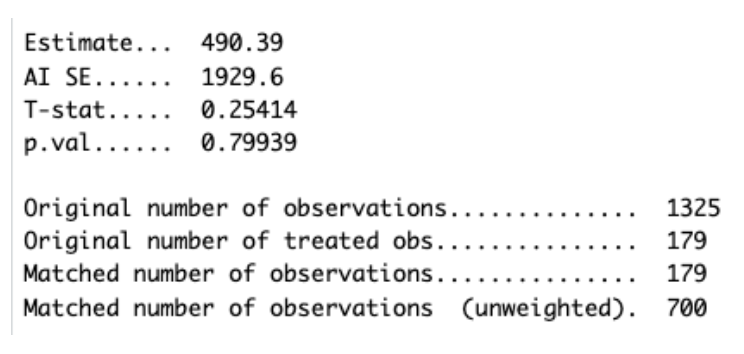
\includegraphics[width=0.4\textwidth]{figures/q7_f.png}
       \caption{Snapshot of output produced by running \texttt{symmary()} on the object returned by \texttt{Matching::Match()} in \textbf{\ref{item:estimate-att-ncs}}.}
       \label{fig:nnm_output}
       \end{figure}
\end{enumerate}

\textbf{Solution:} This line means that there are 700 matched pairs.
This does not take into account that one treated unit might be matched
with multiple control units.

\begin{enumerate}
\def\labelenumi{\alph{enumi}.}
\setcounter{enumi}{6}
\tightlist
\item
  (2 p) Use the matched data to ``manually'\,' compute the ATT estimate.
\item
  (2 p) Run \texttt{Matching::Match()} with \texttt{ties = FALSE}. Why
  do you get
  ``\texttt{Matched number of observations (unweighted). 179}?'\,'
\end{enumerate}

\begin{Shaded}
\begin{Highlighting}[]
\NormalTok{matched\_notie }\OtherTok{\textless{}{-}}\NormalTok{ Matching}\SpecialCharTok{::}\FunctionTok{Match}\NormalTok{(Y,Tr,X,}\AttributeTok{M=}\DecValTok{1}\NormalTok{,}\AttributeTok{estimand=}\StringTok{"ATT"}\NormalTok{,}\AttributeTok{ties =} \ConstantTok{FALSE}\NormalTok{)}
\NormalTok{(}\FunctionTok{summary}\NormalTok{(matched\_notie))}
\end{Highlighting}
\end{Shaded}

\begin{verbatim}
## 
## Estimate...  473.95 
## SE.........  780.81 
## T-stat.....  0.607 
## p.val......  0.54385 
## 
## Original number of observations..............  1325 
## Original number of treated obs...............  179 
## Matched number of observations...............  179 
## Matched number of observations  (unweighted).  179
\end{verbatim}

\textbf{Solution:} I get ``Matched number of observations (unweighted).
179'' because setting ties = FALSE instructs the algorithm not to match
treated units to more than one control unit when there are ties in the
matching criterion (e.g.~distance based on propensity score). So we get
exactly 179 matched pairs.

\textcolor{gray}{\textbf{Programming Guidance}: Explore the list returned by \texttt{Matching::Match()}, in particular the named elements \texttt{mdata}, \texttt{index.treated}, \texttt{index.control} and \texttt{weights}.}
\textcolor{gray}{\textbf{Hint}: Use \texttt{names()} to see the elements in the list returned by \texttt{Matching::Match()}. Feel free to use Table \ref{tab:matched-set-ds} to check on your work on the matched data. The matched data shall be a dataframe with 700 rows, because there are 700 matched pairs. We recommend that you have as columns the following: an index counter for the treated unit in the pair, an index counter for the control unit in the pair, the pscore value for the treated unit in the pair, the pscore value for the control unit in the pair, the outcome (namely \texttt{re78}) for the treated unit in the pair, the outcome for the control unit in the pair, the weight for the control unit in the pair. With this information you can answer all the questions (and more).}

\newpage 
\begin{table}[h]
\centering
\begin{tabular}{|c|c|c|c|c|c|}
\hline
\textbf{\texttt{num\_matches}} & \textbf{\texttt{num\_treated}} & \textbf{\texttt{min\_pscore}} & \textbf{\texttt{avg\_pscore}} & \textbf{\texttt{med\_pscore}} & \textbf{\texttt{max\_pscore}} \\ \hline
209 & 1 & 0.000652575 & 0.000652575 & 0.000652575 & 0.000652575 \\ \hline
129 & 1 & 0.003290713 & 0.003290713 & 0.003290713 & 0.003290713 \\ \hline
70 & 1 & 0.005570029 & 0.005570029 & 0.005570029 & 0.005570029 \\ \hline
35 & 2 & 0.007592412 & 0.007776318 & 0.007776318 & 0.007960224 \\ \hline
9 & 1 & 0.055467716 & 0.055467716 & 0.055467716 & 0.055467716 \\ \hline
7 & 1 & 0.028241882 & 0.028241882 & 0.028241882 & 0.028241882 \\ \hline
5 & 2 & 0.07015485 & 0.082214016 & 0.082214016 & 0.094273183 \\ \hline
4 & 2 & 0.046380154 & 0.061290142 & 0.061290142 & 0.076200129 \\ \hline
3 & 3 & 0.133671949 & 0.688292564 & 0.965164821 & 0.966040924 \\ \hline
2 & 14 & 0.127383235 & 0.369653196 & 0.336881761 & 0.949418099 \\ \hline
1 & 151 & 0.141036436 & 0.753198139 & 0.900426437 & 0.972637597 \\ \hline
\end{tabular}

\caption{Descriptive statistics for the matched data. The column \texttt{num\_matches} lists the (distinct) count of control units matched to a treated unit, from largest to smallest. The column \texttt{num\_treated} reports the number of treated units with the corresponding count of matched controls. The sum of this column is 179, i.e., the number of treated units in the trimmed sample. The sum of the row-wise product of the first two columns is 700. The remaining columns present min/average/median and max value of the pscore for the treated units with the corresponding count of matched controls. Example A: 1 treated unit is matched to 209 distinct control units, this unit's pscore is 0.000652575. Example B: 14 treated units are each matched to exactly two control units, the maximum pscore among these 14 units is 0.949418099. Example C: 151 treated units are each matched to exactly one control unit, the average of these treated units' pscores is 0.753198139.}
\label{tab:matched-set-ds}
\end{table}

\begin{enumerate}
\def\labelenumi{\arabic{enumi}.}
\setcounter{enumi}{7}
\tightlist
\item
  (10 p) Use \texttt{Matching::MatchBalance()} to document balance in
  the covariates (those in the Logit specification for the pscore model)
  before and after matching. Comment on your findings: a) Are covariates
  more/less balanced after matching? b) Are covariates in the matched
  sample sufficiently balanced to make you trust that the NNM estimator
  is not confounded by differences in observables?

  \textcolor{gray}{\textbf{Programming guidance:} Use 500 bootstrap replication, i.e., set \texttt{nboots=500}. Say that you name \texttt{nnm\_balance} the object (a list of lists) returned by the call to \texttt{Matching::MatchBalance()}. Apply \texttt{names()} to see the named element of the list. To check that your implementation is correct: the averages of \texttt{age} in the trimmed sample before matching and in the matched sample (i.e., after matching) are, respectively:
   \begin{itemize}
   \item \texttt{nnm\_balance\$BeforeMatching[[age\_loc]]\$mean.Tr = 25.76536}, 
   \item \texttt{nnm\_balance\$BeforeMatching[[age\_loc]]\$mean.Co = 30.96161},
   \item \texttt{nnm\_balance\$AfterMatching[[age\_loc]]\$mean.Tr = 25.76536},
   \item \texttt{nnm\_balance\$AfterMatching[[age\_loc]]\$mean.Co = 26.1724}
   \end{itemize}
  where, in our script, \texttt{age\_loc} is the number that identifies the location of the information for the covariate \texttt{age}.}
\item
  (6 p) The estimate of ATT based on the experimental data is \$1,794
  with SE \$633 (see PSet 3). Consider the estimates of ATT in Table
  \ref{tab:Tab25-4_2}: What are the takeaways? Taking inspiration from
  Imbens (2015)'s recommendations, are there actions you may want to
  take to gain more confidence in your ability to learn about the true
  causal impact of the offer of training via matching when you only have
  access to observational data?
\end{enumerate}

\newpage
\begin{figure}[!htb]
\centering
  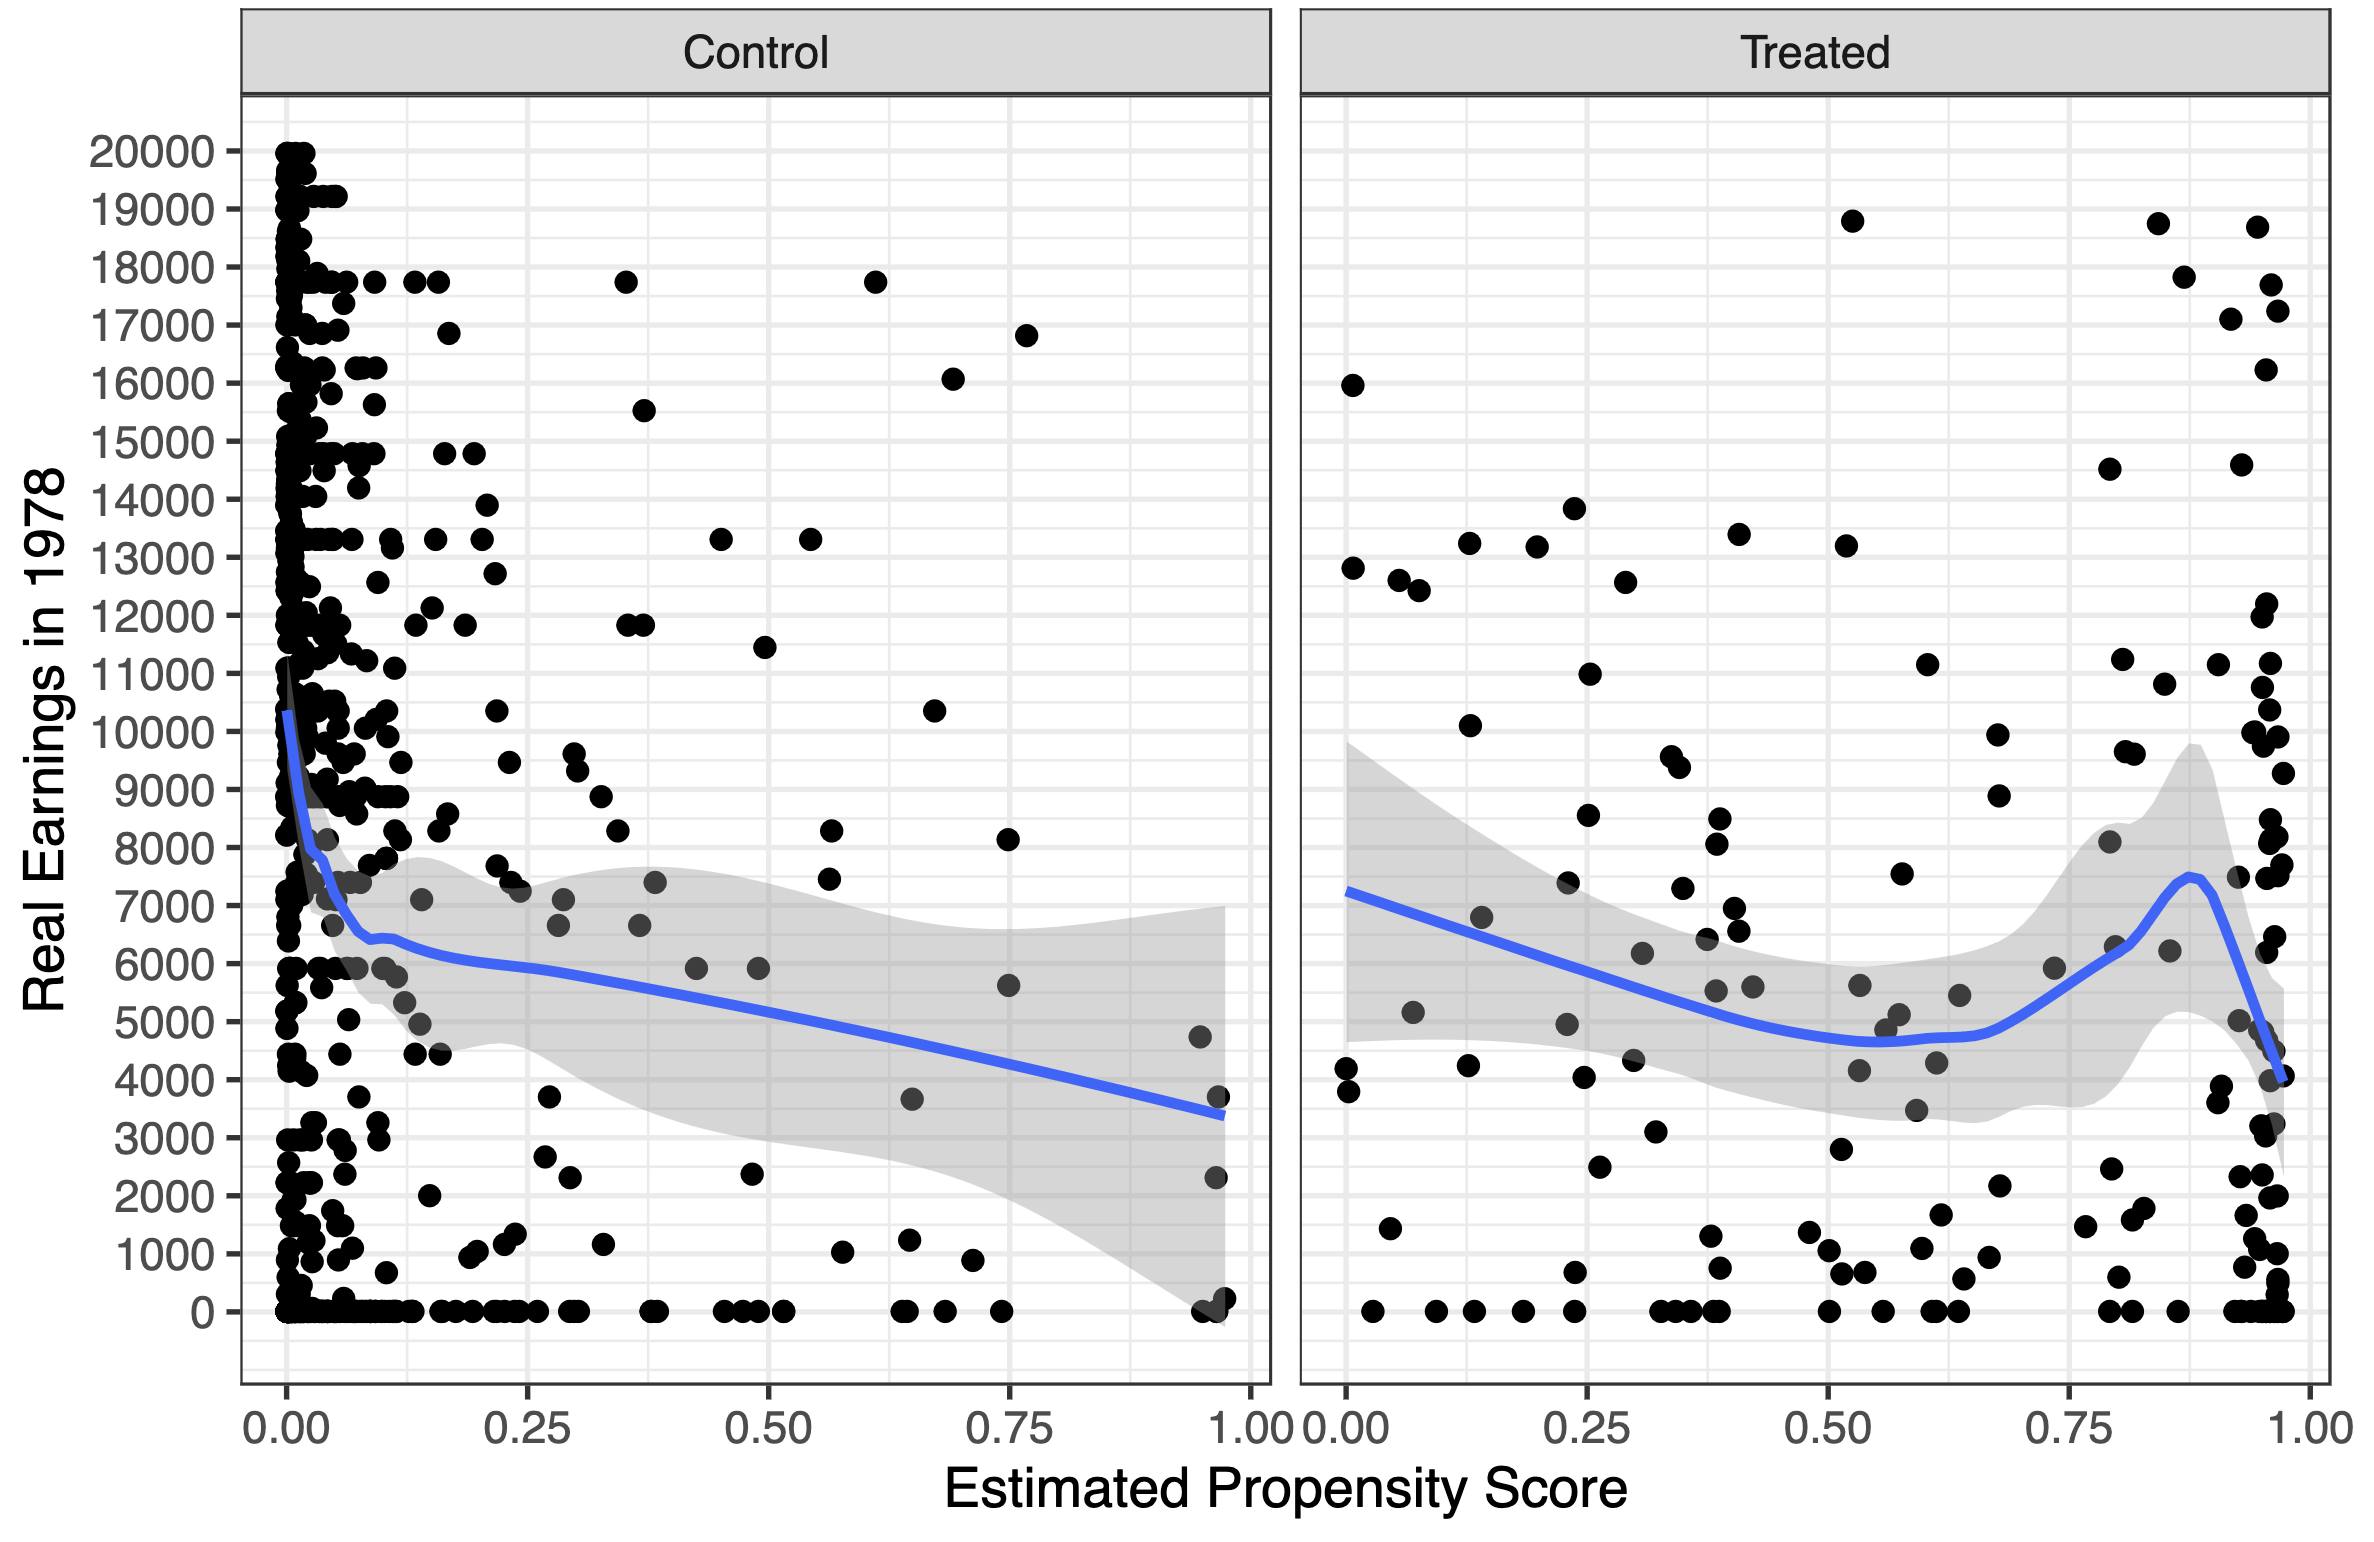
\includegraphics[width=0.9\textwidth]{figures/figures_end.png}
  \caption{Scatter plot of \texttt{re78} against the Logit-based $\widehat{p}_{i}$ estimates, separately for the treated and the control group. Each panel also includes a fitted non-parametric regression of \texttt{re78} on $\widehat{p}_{i}$ (blue line).}
  \label{fig:propensity_vs_earnings}
\end{figure}

\end{document}
